\begin{comment}
    In this section, you introduce the work to your audience.
Even though this is the first chapter of your thesis, you should not necessarily write this chapter first.
It is often easier to write this chapter at the end of the thesis writing.
In this part of your introduction, i.e., the part before the Motivation section (\autoref{sec:intro_ssec:motiv}), you write a paragraph (not just a sentence) for each of the bullet points mentioned in the abstract:

\begin{itemize}
	\item Domain, i.e., explain the application domain in which your thesis is applicable.
	\item Problem, i.e., motivate what the problem is you are solving.
	\item Method, i.e., describe the method you have proposed, and, compare it, briefly \& high level to other approaches. In particular, focus on the benefits of your approach versus the other approach(es)
	\item Evaluation, i.e., how did you evaluate your method and what do the results indicate?
\end{itemize}

Optionally, you can finalize this part with a little overview of what is still to come in this chapter:
\enquote{The remainder of this chapter is structured as follows.
In \autoref{sec:intro_ssec:motiv}, we motivate the need for \dots
In \autoref{sec:intro_ssec:probs}, we provide a formal problem statement.
\dots
}

Before we dive into the motivation section, a few general guidelines for writing:
\begin{enumerate}
	\item Write \emph{active} and in the \emph{present tense}.
	\item Avoid \enquote{optionality} as much as possible, i.e., usage of the following words should (pun intended) be minimized:
	\begin{itemize}
		\item could
		\item would
		\item should
		\item may
		\item might
		\item can
		\item will
		\item ...
	\end{itemize}
	Good: We present a method that ...\\
	Bad: We will present a method that ...\\
	Good: We use function $f$ and compute its inverse.\\
	Bad: We can use the function $f$ and will compute its inverse.\\
	\item Connect mathematical operators using the \{ \}-operators in math mode (\$ \$).\\
	Good: $x{\in}X$\\
	Bad: $x \in X$\\
	Good: $f{\colon}X{\to}Y$\\
	Bad: $f \colon X \to Y$\\
	If using \{ \} prevents your mathematics to break at the end of the line, use \texttt{$\backslash$allowbreak} in math mode.
	\item Do not use $\backslash\backslash$ to generate line breaks % we used a few before, however do not use them in text!
	
	Do it like

	This
	\item Position the caption of a Figure below the figure.
	\item Position the caption of a Table above the table.
	\item Write Section Headings and Titles Like This\\
	Good: Approximation Bias in Unstable Systems\\
	Bad: Approximation bias in unstable systems\\
	\item Be consistent in your references.
	\begin{itemize}
		\item Make sure that the name of the same author is always the same (using DBLP helps for this)
		\item Titles should be consistent. Either use the style previously described, i.e., Approximation Bias in Unstable Systems or Approximation bias in unstable systems (this is allowed in the references, opposed to your own section headings and titles, however, \emph{BE CONSISTENT}).
	\end{itemize}
\end{enumerate}
\item Next steps: Develop a library to play-out translucent logs from a process model (petri net).
\end{comment}

\section{Motivation}
\label{sec:intro_ssec:motiv}

\begin{comment}
    In this section, you explain to the reader why:

\begin{enumerate}
    \item The problem you are solving is relevant to be solved.
    \item The existing solutions do not solve the problem and/or have significant problems/shortcomings when doing so.
\end{enumerate}
Note that parts of this section are already highlighted in both the abstract and the introduction.
However, in this section, you dive a bit deeper.
In a good motivation, you show a (simple) example on which current methods fail, yet, the method that you are going to describe in this thesis actually yields a better result.

For example, assume that your thesis describes a new \emph{process discovery} algorithm that is able to handle noise, incomplete behavior, and, on top of that, is able to apply label-splitting.
You can take an (example) event log and show that existing algorithms result in models that are of suboptimal quality.
Finally, you show a model discovered by your fancy algorithm, and, you explain why this model is so much better.
\end{comment}

Business processes are seldom linear. Instead, they are usually a messy, chaotic, intertangled mash of activities where its golden path is meticulously hidden. On top of that, event logs have no guarantee of completeness. The quality of the process model therefore is entirely dependent on the quality of its event log.

An ideal event log would be \emph{transparent}, containing metadata of structural properties of the corresponding process model, e.g. state information in a Petri net setting. Event logs, however, are usually \emph{opaque} - one cannot identify the underlying process model straight away by solely looking at the log. One must instead utilize process discovery algorithms to generate corresponding models. By its nature, process discovery algorithms primarily focus on what \emph{happened}. However, they often do not take into consideration what \emph{could have happened} instead. An event log is \textit{translucent} if the log contains the information which potential, alternative realities of the past could have occurred instead of the activity occurred in the real world. Logs of this nature are called \textit{translucent event logs.} and are extremely beneficial to enhance the quality of existing process discovery algorithms.

Let us consider a small example as motivation. Suppose the underlying model of our business process is represented as the petri net below.

\begin{figure}[h]
    \centering
    \begin{tikzpicture}
    % Place 1
    \node[place, tokens=1] (p1) at (0,0) {};
    
    % Place 2
    \node[place] (p2) at (3,1) {};

    % Place 3
    \node[place] (p3) at (3,-1) {};

    % Place 4
    \node[place] (p4) at (6,1) {};

	% Place 5
	\node[place] (p5) at (6,-1) {};

    % Place 6
    \node[place] (p6) at (9,0) {};
    
    % Transition a
    \node[transition, minimum width=0.8cm, minimum height=0.8cm, label=center:a] (a) at (1.5,0) {}
        edge[pre]   (p1)
        edge[post]  (p2)
        edge[post]  (p3);
        
    % Transition b
    \node[transition, minimum width=0.8cm, minimum height=0.8cm, label=center:b] (b) at (4.5,1) {}
        edge[pre]   (p2)
        edge[post]  (p4);

    % Transition c
    \node[transition, minimum width=0.8cm, minimum height=0.8cm, label=center:c] (c) at (4.5,-1) {}
        edge[pre]   (p3)
        edge[post]  (p5);
        
    % Transition d
    \node[transition, minimum width=0.8cm, minimum height=0.8cm, label=center:d] (d) at (7.5,0) {}
        edge[pre]   (p4)
		edge[pre]   (p5)
        edge[post]  (p6);
\end{tikzpicture}
\caption{Example business model represented as a petri net.}
\label{petrinet}

\end{figure}

We play-out the model fifty times and retrieve the event log $\mathcal{L}_1 = [ \langle a, b, c, d \rangle ^{48}, \langle a, c, b, d \rangle^2 ]$ in the process. We can then leverage widely used process discovery algorithms to rediscover the process model described in Figure \ref{petrinet}. 

This works under the assumption of log completeness, but what would happen if the trace $\langle a, c, b, d \rangle$ occurs so rarely that we weren't able to capture the behavior? Given the incomplete log $\mathcal{L}_1 = [ \langle a, b, c, d \rangle ^{50}]$, every process discovery algorithm will return a linear process model. The translucent variant would look like $\mathcal{L}_2 = [ \langle \underline{a}, \underline{b}c,  \underline{c},  \underline{d} \rangle ^{50}]$, where all enabled activities are listed and the executed activity is underscored. Here, the choice situation between activities $b$ and $c$ is clearly visible, thus preventing the linear modelling of our process.

% % In fact, translucent logs make the process discovery trivial for a certain subclass of process models, for which each state activates a unique set of activities. Such process models are called \textit{lucent process models.} Sound workflow nets that are short-circuited and free-choice belong to this class of process models. Although this seems like a hard restriction, many of the real-life workflow nets modelling business processes are reported to possess the free-choice property \cite{Advances in Quantitative Analysis of Free-Choice Workflow Petri Nets}.

Despite its benefits, lucent models and translucent event logs are relatively new concepts and are therefore scarcely researched. As a result, translucent event logs are hardly available in real-life process logs. This motivates us to devise novel methods to generate translucent event logs from a non-translucent variant.

\section{Problem Statement}
\label{sec:intro_ssec:probs}

\begin{comment}
    In this section, you introduce the problem that you are solving.
A good problem statement is a concise, more general statement of the example motivation that you have used in the motivation section.

For example, in the case of our previous example:

\enquote{Real event data contains infrequent and incomplete behavior. 
Furthermore, different recordings of the same activity may refer to conceptually different contextual executions.
Existing, state-of-the-art process discovery algorithms cannot discover process models of adequate quality, given event data of the previously described form.}
\end{comment}

\begin{figure}
    \centering
    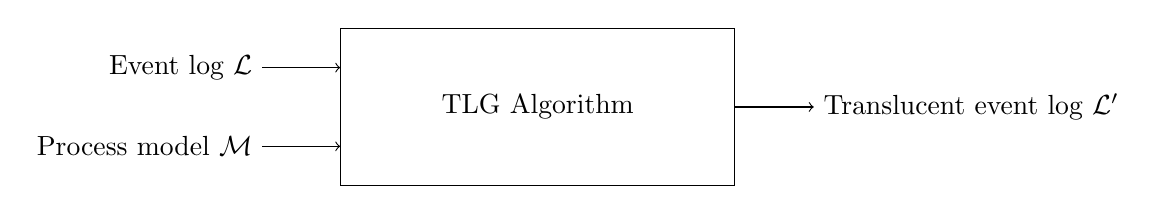
\begin{tikzpicture}

    % Draw the box
    \node[draw, minimum width=5cm, minimum height=2cm, align=center] (box) at (0,0) {TLG Algorithm};

    % Draw the input arrows with labels on the side
    \draw[->] (-3.5,0.5) -- node[pos=0,left] {Event log $\mathcal{L}$} (box.west |- 0.5, 0.5);
    \draw[->] (-3.5,-0.5) -- node[pos=0, left] {Process model $\mathcal{M}$} (box.west |- -0.5,-0.5);

    % Draw the output arrow with label on the side
    \draw[->] (box.east) -- ++(1,0) node[right] {Translucent event log $\mathcal{L'}$};

\end{tikzpicture}
    \caption{Translucent Log Generation Problem.}
    \label{fig:enter-label}
\end{figure}


In order to look deeper into the main problem of this thesis, we first formally define our problem as described below. \\

\begin{definition}[Translucent Log Generation Problem]
\label{def:tlgp}
    Given an event log $\mathcal{L}$ as input, produce a translucent event log $\mathcal{L'}$ where the set of enabled activities are added as attributes. 
\end{definition}

There is a variant of the \emph{Translucent Log Generation Problem}, where a process model is provided along with the event log. \\

\begin{definition}[Translucent Log Generation Problem - Process Model Variant]
\label{def:tlgpm}
    Given an event log $\mathcal{L}$ and a process model $\mathcal{M}$ as inputs, produce a translucent event log $\mathcal{L'}$ where the set of enabled activities are added as attributes. 
\end{definition}

The second variant differs from the first, as the set of enabled activities is constrained by the process model. Note that the function of $\mathcal{M}$ is to provide an upper bound on the set of enabled activities, and the log is there to provide further constraints to enrich the model. Of particular interest are parallel and choice situations, since we are able to deduce supplementary patterns not demonstrated in the process model using log data. We name the first variant defined in Definition \ref{def:tlgp} as \emph{Bottom-up Translucent Log Generation Problem}, whereas the second variant in Definition \ref{def:tlgpm} is named as \emph{Top-down Translucent Log Generation Problem.}

\section{Research Questions}
\begin{comment}
    The research questions you pose, are questions you need to (largely) answer in order to solve the problem.
Basically, the combined set of answers to the questions you pose, allow you to solve the research problem.

From the book of Justin Zobel, \enquote{Writing for Computer Science}~\cite{DBLP:books/sp/Zobel14} (which we highly recommend you to read before writing):

\enquote{
	A hypothesis or research question should be specific and precise, and should be
	unambiguous; the more loosely a concept is defined, the more easily it will satisfy
	many needs simultaneously, even when these needs are contradictory. And it is
	important to state what is not being proposed—what the limits on the conclusions
	will be.
}

In the context of our example, we can define many relevant research questions:
\begin{enumerate}
	\item What are typical prominent noise patterns in real event data?
	\item How to detect noise patterns in event data?
	\item How to detect infrequent behavior in event data?
	\item How to detect contextually different executions of the same activity?
	\item How to balance between detected noise patterns, infrequent behavior and imprecise labels?
	\item 
\end{enumerate}
Typically, your thesis consists of 3-5 research questions (often multiple more questions can be defined).
\end{comment}

In the scope of the thesis, we define the five research questions below: 

\textbf{(RQ1.)} Which techniques can be derived to tackle the \textit{Translucent Log Generation Problem}?

\textbf{(RQ2.)} How can we guarantee the accuracy of predictions made by our algorithm?

\textbf{(RQ3.)} How much value do the novel techniques add compared to the state-of-the-art process discovery algorithms?

\textbf{(RQ4.)} How can the data-centered aspect be incorportaed in our method?

\textbf{(RQ4.)} How should we design and implement an intuitive, user-friendly tool to demonstrate our results?



\section{Research Goals}
\begin{comment}
    In this section, you present your research goals.
A research goal is a concise statement that s.t., achieving the goal helps you in (partially) solve a research question.
Hence, the research questions and goals are often very related.
Furthermore, it should be obvious for the reader what goal answers what problem.

In the context of our previously mentioned questions, some example goals are:
\begin{itemize}
	\item Conduct a systematic literature review on noise patterns in real event data.
	\item Design a noise detection algorithm.
	\item Formalize the notion of incompleteness in an event log.
	\item ...
\end{itemize}
\end{comment}

The principal research goal is to develop a framework dedicated to solve the \emph{Translucent Log Generation Problem} with the following properties:

\begin{enumerate}
    \item Accurately reflects the enabled activities
    \item Performs well regarding time complexity, particularly with large event logs
    \item Easily operable for end-users
\end{enumerate}

By building a meaningful framework, our framework should add value to enhancing existing process discovery algorithms with more accurate models.

% \section{Contributions}
\begin{comment}
    In this section, you list the contributions that your thesis makes to our wonderful world (of science).
Again, there is a strong link to the previous section.
Usually, you have achieved your research goals.
Hence, the contributions are concrete statements of the goals you have achieved.
Additionally, your evaluation (most likely also stressed as a goal) is a contribution.
Any implementation or prototype can also be quantified as a contribution.

Some examples:
\begin{itemize}
	\item A systematic literature review covering 35 articles on noise patterns in real event data
	\item A noise detection algorithm based on dynamic programming and symbolic linking
	\item ...
\end{itemize}
\end{comment}


% \section{Thesis Structure}

% The remainder of this thesis is structured as follows. We first present basic mathematical preliminaries in \autoref{chap:prelim}. Related work is presented in \autoref{chap:related_work}. In \autoref{chap:method}, the main ideas of translucent event log generation algorithms are presented and thoroughly explained, followed by the implementation specifications in \autoref{chap:impl}. The evaluation methods and results are displayed in \autoref{chap:eval}. Finally, discussion of the result, further limitations and future perspectives are presented in \autoref{chap:discussion}. 